\section{Le SQL vs le NoSQL:}
Dans un but d'analyse et de comparaison (SQL vs NoSQL), il nous a été demandé de réaliser le modèle E-A relative a notre cas d'étude que nous présenterons ci-dessous ainsi que le modèle relationnel:

\subsection{Le modèle entité association:}


\subsection{Le modèle relationnel:}
Le modèle relationnel est une manière de représenter les relations existantes entre plusieurs informations, et de les ordonner entre elles.
A partir du modèle E-A précédent, on peut faire un passage vers le modèle relationnel en respectant les règles de passage et on obtient le modèle relationnel suivant :

\begin{figure}[h]
	\centering
	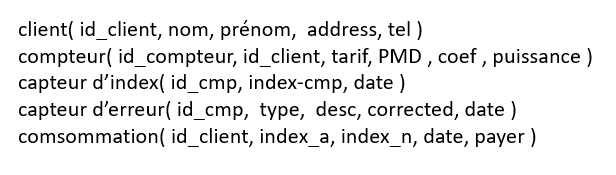
\includegraphics[scale=1]{img/part2/2.6.png}
	\caption{Le modèle relationnel}
\end{figure}
